\documentclass[12pt,a4paper]{article}
\usepackage[utf8]{vietnam}
\usepackage{amsmath,amssymb}
\usepackage{geometry}
\geometry{top=1.5cm,bottom=1.2cm,left=1.4cm,right=1.4cm,headheight=28pt,headsep=12pt,footskip=18pt}
\usepackage{tikz}
\usepackage{xcolor}
\usepackage{enumerate}
\usepackage{graphicx}
\usepackage[version=4]{mhchem}
\usepackage{fancyhdr}
\usepackage{ex_test}

\renewcommand{\baselinestretch}{0.96}
\setlength{\parskip}{0pt}

\definecolor{hfRed}{RGB}{211,47,47}
\definecolor{hfGreen}{RGB}{139,195,144}

\providecommand{\False}{}

\pagestyle{fancy}
\fancyhf{}
\fancyhead[L]{\small\itshape\color{hfRed} Tài liệu lưu hành nội bộ}
\fancyhead[R]{\small\itshape\color{hfRed} Thầy \textbf{TRẦN VĂN THẠNH} - 0777.470.803}
\renewcommand{\headrulewidth}{0.8pt}
\renewcommand{\headrule}{\hbox to\headwidth{\color{hfGreen}\leaders\hrule height \headrulewidth\hfill}}

\fancyfoot[L]{\small\itshape\color{hfRed} CS1: 6/15 Nguyễn Hoàng, P. Kim Long, TP Huế \quad|\quad CS2: 24 Đặng Thái Thân, TP Huế}
\fancyfoot[R]{\small\bfseries\color{hfRed} Trang \thepage}
\renewcommand{\footrulewidth}{0.8pt}
\renewcommand{\footrule}{\hbox to\headwidth{\color{hfGreen}\leaders\hrule height \footrulewidth\hfill}}

\fancypagestyle{firstpage}{
  \fancyhf{}
  \renewcommand{\headrulewidth}{0pt}
  \fancyfoot[L]{\small\itshape\color{hfRed} CS1: 6/15 Nguyễn Hoàng, P. Kim Long, TP Huế \quad|\quad CS2: 24 Đặng Thái Thân, TP Huế}
  \fancyfoot[R]{\small\bfseries\color{hfRed} Trang \thepage}
  \renewcommand{\footrulewidth}{0.8pt}
  \renewcommand{\footrule}{\hbox to\headwidth{\color{hfGreen}\leaders\hrule height \footrulewidth\hfill}}
}

\begin{document}
\thispagestyle{firstpage}

\noindent
\begin{minipage}[t]{0.44\textwidth}
	\centering\fontsize{10pt}{12pt}\selectfont
	\textbf{SỞ GIÁO DỤC VÀ ĐÀO TẠO THỪA THIÊN HUẾ}\\
	\textbf{ĐỀ CHÍNH THỨC}\\
	\textit{(Đề thi có 04 trang)}
\end{minipage}\hfill
\begin{minipage}[t]{0.54\textwidth}
	\centering\small
	\textbf{ĐỀ KIỂM TRA ĐỊNH KỲ CHƯƠNG 1 (ESTER -- LIPID)}\\
	\textbf{MÔN: HOÁ HỌC -- LỚP 12}\\
	\textit{Thời gian làm bài: 50 phút (không kể thời gian phát đề)}\\
	\fbox{\textbf{MÃ ĐỀ: 102}}
\end{minipage}

\smallskip
\begin{center}
	{\color{hfRed}\textbf{\large (BẢN GIÁO VIÊN -- CÓ LỜI GIẢI CHI TIẾT)}}
\end{center}

\smallskip
\noindent\hrulefill
\smallskip

\noindent\textbf{Họ, tên thí sinh:} \dotfill\ \textbf{Lớp:} \dotfill\ \textbf{Số báo danh:} \dotfill

\smallskip
\noindent\textit{(Cho biết nguyên tử khối: H = 1; C = 12; N = 14; O = 16; Na = 23; K = 39; Br = 80; Cl = 35,5).}
\smallskip

\noindent
\textbf{PHẦN I (4,5 điểm -- 18 câu): Câu trắc nghiệm nhiều phương án lựa chọn.}\\
\textit{Thí sinh trả lời từ câu 1 đến câu 18. Mỗi câu hỏi thí sinh chỉ chọn một phương án.}

\Opensolutionfile{ans}[ans-de02gv]

\begin{ex}
$\ce{HCOOCH3}$ được sử dụng làm dung môi cho nitrocellulose và cellulose acetate, một chất trung gian trong sản xuất dược phẩm và thuốc xông hơi. Tên gọi của $\ce{HCOOCH3}$ là
\choice
{ethyl formate}
{ethyl acetate}
{\True methyl formate}
{methyl acetate}
\loigiai{
$\ce{HCOOCH3}$ gồm gốc acid formate ($\ce{HCOO-}$) và gốc alkyl methyl ($-\ce{CH3}$), có tên gọi là \textbf{methyl formate}.\\
\textbf{Chọn C.}}
\end{ex}

\begin{ex}
Ester nào sau đây tác dụng với $\ce{NaOH}$ thu được ethyl alcohol?
\choice
{\True $\ce{CH3COOC2H5}$}
{$\ce{CH3COOC3H7}$}
{$\ce{C2H5COOCH3}$}
{$\ce{HCOOCH3}$}
\loigiai{
Phản ứng: $\ce{CH3COOC2H5 + NaOH ->[t^\circ] CH3COONa + C2H5OH}$. $\ce{C2H5OH}$ là ethyl alcohol.\\
\textbf{Chọn A.}}
\end{ex}

\begin{ex}
Công thức tổng quát của ester mạch hở được tạo thành từ carboxylic acid no, đơn chức và alcohol no, đơn chức là
\choice
{$\ce{C_{n}H_{2n-1}COOC_{m}H_{2m+1}}$}
{$\ce{C_{n}H_{2n-1}COOC_{m}H_{2m-1}}$}
{$\ce{C_{n}H_{2n+1}COOC_{m}H_{2m-1}}$}
{\True $\ce{C_{n}H_{2n+1}COOC_{m}H_{2m+1}}$}
\loigiai{
Carboxylic acid no, đơn chức có gốc $\ce{C_{n}H_{2n+1}-}$ ($n \ge 0$), alcohol no, đơn chức có gốc $-\ce{C_{m}H_{2m+1}}$ ($m \ge 1$). Công thức là $\ce{C_{n}H_{2n+1}COOC_{m}H_{2m+1}}$.\\
\textbf{Chọn D.}}
\end{ex}

\begin{ex}
Chất X có công thức cấu tạo $\ce{CH3CH2COOCH3}$ là một chất lỏng trong suốt với mùi trái cây và mùi thơm của rum. Tên gọi của X là
\choice
{propyl acetate}
{\True methyl propionate}
{methyl acetate}
{ethyl acetate}
\loigiai{
$\ce{CH3CH2COOCH3}$ gồm gốc propionate ($\ce{CH3CH2COO-}$) và methyl ($-\ce{CH3}$). Tên gọi là \textbf{methyl propionate} (hoặc methyl propanoate).\\
\textbf{Chọn B.}}
\end{ex}

\begin{ex}
Thủy phân methyl propanoate trong môi trường acid thu được sản phẩm gồm:
\choice
{$\ce{CH3COOH}$ và $\ce{C3H7OH}$}
{$\ce{CH3COOH}$ và $\ce{C2H5OH}$}
{$\ce{C2H5COOH}$ và $\ce{C2H5OH}$}
{\True $\ce{C2H5COOH}$ và $\ce{CH3OH}$}
\loigiai{
Phương trình: $\ce{C2H5COOCH3 + H2O <=>[\ce{H+}, t^\circ] C2H5COOH + CH3OH}$.\\
\textbf{Chọn D.}}
\end{ex}

\begin{ex}
Công thức nào sau đây có thể là công thức của chất béo?
\choice
{$\ce{CH3COOCH2C6H5}$}
{$\ce{C15H31COOCH3}$}
{$\ce{(C17H33COO)2C2H4}$}
{\True $\ce{(C17H35COO)3C3H5}$}
\loigiai{
Chất béo là triester của glycerol với các acid béo, có dạng $\ce{(RCOO)3C3H5}$. $\ce{(C17H35COO)3C3H5}$ (tristearin) là chất béo.\\
\textbf{Chọn D.}}
\end{ex}

\begin{ex}
Acid nào sau đây là acid béo?
\choice
{formic acid}
{\True oleic acid}
{acrylic acid}
{acetic acid}
\loigiai{
Acid béo là carboxylic acid đơn chức, mạch carbon dài, không phân nhánh, thường có số C chẵn. Oleic acid ($\ce{C17H33COOH}$) là acid béo.\\
\textbf{Chọn B.}}
\end{ex}

\begin{ex}
Chất không phải acid béo là
\choice
{\True acetic acid}
{palmitic acid}
{stearic acid}
{oleic acid}
\loigiai{
Acetic acid ($\ce{CH3COOH}$) chỉ có 2 nguyên tử carbon trong phân tử nên không phải acid béo.\\
\textbf{Chọn A.}}
\end{ex}

\begin{ex}
Hỗn hợp các muối sodium của acid béo sinh ra ở trạng thái keo. Để tách muối này ra khỏi hỗn hợp, người ta thêm chất gì vào hỗn hợp?
\choice
{tinh bột}
{\True muối ăn}
{nước}
{acid}
\loigiai{
Thêm dung dịch $\ce{NaCl}$ bão hoà (muối ăn) làm tăng khối lượng riêng của dung dịch và làm giảm độ tan của muối acid béo (hiệu ứng muối kết), giúp xà phòng đông tụ và nổi lên trên bề mặt.\\
\textbf{Chọn B.}}
\end{ex}

\begin{ex}
Ester có công thức phân tử là $\ce{C2H4O2}$ được tạo thành từ methyl alcohol và carboxylic acid nào sau đây?
\choice
{propionic acid}
{acetic acid}
{\True formic acid}
{oxalic acid}
\loigiai{
Ester tạo từ $\ce{CH3OH}$ có dạng $\ce{RCOOCH3}$. Với $\ce{C2H4O2} \Rightarrow \ce{R}$ là $\ce{H-}$, công thức là $\ce{HCOOCH3}$ (tạo từ formic acid $\ce{HCOOH}$).\\
\textbf{Chọn C.}}
\end{ex}

\begin{ex}
Hợp chất nào dưới đây được sử dụng làm xà phòng?
\choice
{$\ce{CH3COONa}$}
{\True $\ce{CH3(CH2)14COONa}$}
{$\ce{CH3(CH2)12COOCH3}$}
{$\ce{CH3(CH2)5O(CH2)5CH3}$}
\loigiai{
$\ce{CH3(CH2)14COONa}$ là sodium palmitate ($\ce{C15H31COONa}$), muối của acid béo dùng làm xà phòng.\\
\textbf{Chọn B.}}
\end{ex}

\begin{ex}
Phản ứng xà phòng hóa là phản ứng xảy ra giữa
\choice
{\True chất béo với base}
{chất béo với sulfuric acid đặc}
{chất béo với acid béo}
{chất béo với acid hữu cơ}
\loigiai{
Phản ứng xà phòng hoá là phản ứng thủy phân chất béo (hoặc ester) trong môi trường kiềm (base) đun nóng.\\
\textbf{Chọn A.}}
\end{ex}

\begin{ex}
Chất nào cùng thành phần nguyên tố với chất béo?
\choice
{dầu mỏ}
{\True tinh dầu sả}
{ethylene}
{dầu bôi trơn}
\loigiai{
Chất béo gồm các nguyên tố $\ce{C, H, O}$. Tinh dầu sả chứa các dẫn xuất terpenoid chứa oxygen (geraniol, citronellal có thành phần $\ce{C, H, O}$), cùng thành phần nguyên tố với chất béo. Dầu mỏ, dầu bôi trơn, ethylene chỉ gồm $\ce{C, H}$.\\
\textbf{Chọn B.}}
\end{ex}

\begin{ex}
Nhận định nào sau đây đúng?
\choice
{\True Chất béo là triester của glycerol với acid béo}
{Xà phòng là muối của acid vô cơ}
{Mỡ động vật, dầu thực vật thường tan tốt trong nước}
{Dung dịch xà phòng có môi trường acid}
\loigiai{
Theo định nghĩa: Chất béo là triester của glycerol với các acid béo (triglyceride).\\
\textbf{Chọn A.}}
\end{ex}

\begin{ex}
Cho sơ đồ: $\ce{X + Y ->[t^\circ] \text{Xà phòng} + \text{glycerol}}$. Các chất X, Y có thể lần lượt là
\choice
{alcohol và base}
{\True ester và base}
{base và acid}
{ester và alcohol}
\loigiai{
Chất béo là triester phản ứng với dung dịch base (kiềm) đun nóng tạo xà phòng và glycerol.\\
\textbf{Chọn B.}}
\end{ex}

\begin{ex}
Xét phân tử xà phòng có cấu tạo như hình bên:
\begin{center}
	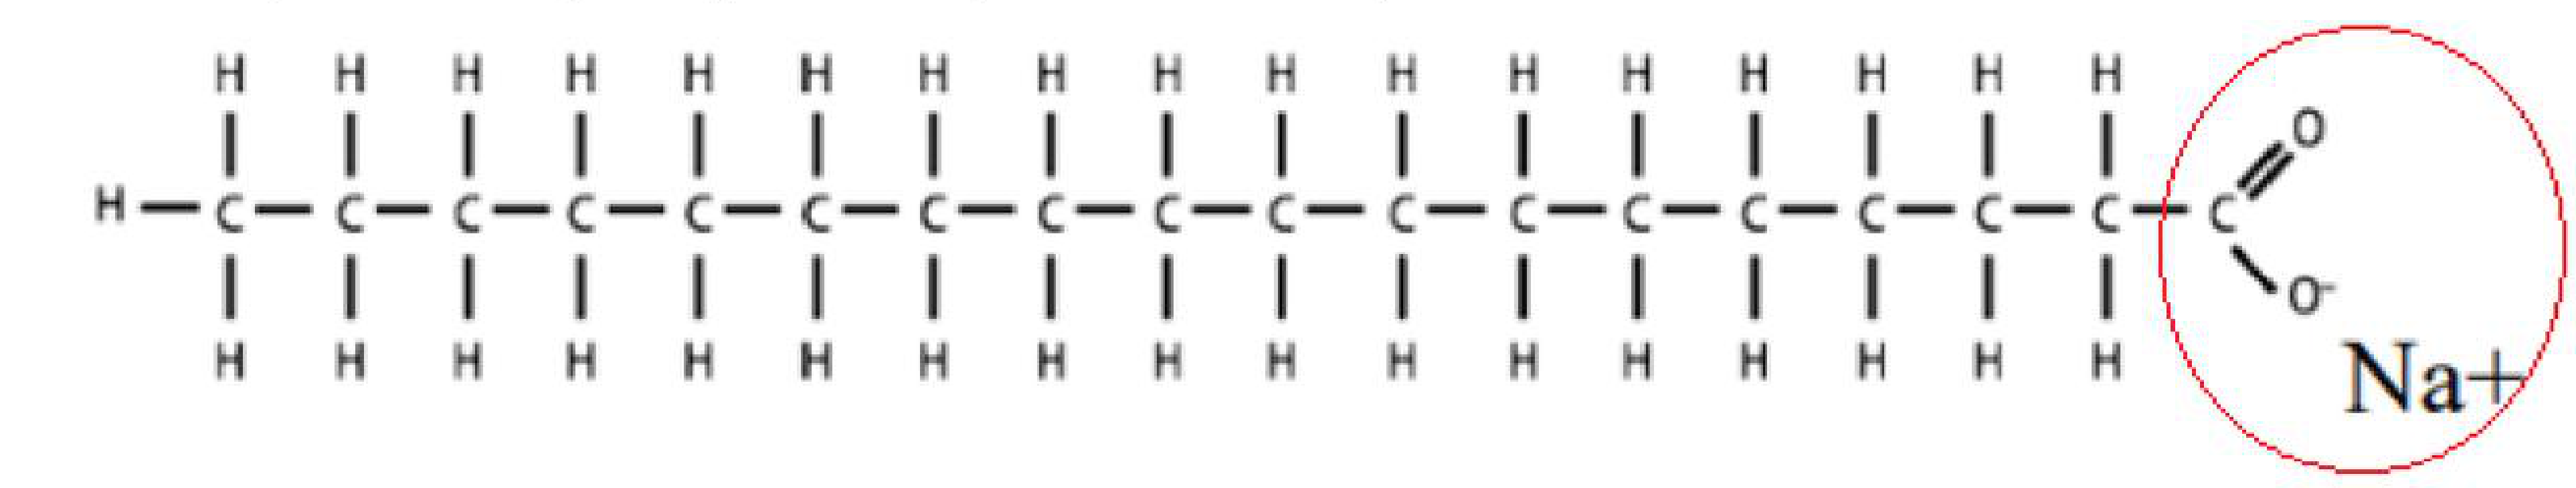
\includegraphics[width=13cm]{images_crop_de02/cau16_phan_tu_xa_phong.png}
\end{center}
Nhóm được khoanh tròn trong công thức trên là
\choice
{nhóm kị nước}
{nhóm dị thể}
{\True nhóm ưa nước}
{nhóm đồng thể}
\loigiai{
Phân tử xà phòng gồm phần đuôi hydrocarbon dài kị nước (ưa dầu mỡ) và nhóm carboxylate mang điện tích âm $-\ce{COO^-Na^+}$ ở đầu là nhóm phân cực ưa nước.\\
\textbf{Chọn C.}}
\end{ex}

\begin{ex}
Thể tích $\ce{H2}$ (đkc) cần để hydrogen hóa hoàn toàn $1\text{ tấn}$ triolein là
\choice
{\True $84128{,}96\text{ L}$}
{$760{,}18\text{ lít}$}
{$7{,}6018\text{ lít}$}
{$7601{,}8\text{ lít}$}
\loigiai{
$M_{\text{triolein}} = 884\text{ g/mol}$; $n_{\text{triolein}} = \dfrac{10^6}{884} \approx 1131{,}2217\text{ mol}$.\\
$\ce{(C17H33COO)3C3H5 + 3H2 ->[Ni, t^\circ] (C17H35COO)3C3H5}$.\\
$n_{\ce{H2}} = 3 \times n_{\text{triolein}} = 3393{,}665\text{ mol}$.\\
$V_{\ce{H2}} = 3393{,}665 \times 24{,}79 \approx \mathbf{84128{,}96\text{ L}}$.\\
\textbf{Chọn A.}}
\end{ex}

\begin{ex}
Cho $1\text{ mol}$ triglyceride X tác dụng với dung dịch $\ce{NaOH}$ dư, thu được $1\text{ mol}$ glycerol, $1\text{ mol}$ sodium palmitate và $2\text{ mol}$ sodium oleate. Phát biểu nào sau đây sai?
\choice
{Phân tử X có 5 liên kết $\pi$}
{Có 2 đồng phân cấu tạo thỏa mãn tính chất của X}
{\True Công thức phân tử chất X là $\ce{C52H96O6}$}
{$1\text{ mol}$ X làm mất màu tối đa $2\text{ mol}$ $\ce{Br2}$ trong dung dịch}
\loigiai{
X có công thức cấu tạo là $\ce{(C15H31COO)(C17H33COO)2C3H5}$.\\
Công thức phân tử của X là $\ce{C55H102O6}$ (chứ không phải $\ce{C52H96O6}$).\\
\textbf{Chọn C.}}
\end{ex}

\Closesolutionfile{ans}

\vspace{0.3cm}
\noindent
\textbf{PHẦN II (4,0 điểm -- 4 câu): Câu trắc nghiệm đúng sai.}\\
\textit{Thí sinh trả lời từ câu 1 đến câu 4. Trong mỗi ý a), b), c), d) ở mỗi câu, thí sinh chọn đúng hoặc sai.}

\setcounter{ex}{0}

\begin{ex}
Cho các phát biểu về acid béo và chất béo sau:
\choiceTF[t]
{\False Acid béo thường có gốc hydrocarbon mạch dài, có số nguyên tử carbon lẻ.}
{\False Khi xà phòng hoá chất béo, sản phẩm thu được là glycerol và các acid đơn chức.}
{\True Chất béo có nhiều gốc acid no thường ở dạng rắn, còn chất béo có nhiều gốc acid không no thường ở dạng lỏng.}
{\False Acid béo omega-3 là các acid béo không no có liên kết đôi đầu tiên ở vị trí số 3 nếu đánh số từ nhóm carboxyl (-COOH).}
\loigiai{
\begin{itemize}
	\item a) \textbf{Sai.} Acid béo hầu hết có số nguyên tử carbon chẵn (12 đến 24C), mạch không phân nhánh.
	\item b) \textbf{Sai.} Phản ứng xà phòng hoá tạo ra glycerol và muối của acid béo (xà phòng), không phải acid đơn chức.
	\item c) \textbf{Đúng.} Gốc acid no (stearin, palmitin) làm chất béo ở dạng rắn; gốc acid không no (olein) làm chất béo ở dạng lỏng.
	\item d) \textbf{Sai.} Đánh số từ nguyên tử carbon của nhóm methyl cuối mạch ($-\ce{CH3}$), gọi là vị trí $\omega$.
\end{itemize}}
\end{ex}

\begin{ex}
Người ta thực hiện phản ứng xà phòng hóa như hình vẽ dưới đây:
\begin{center}
	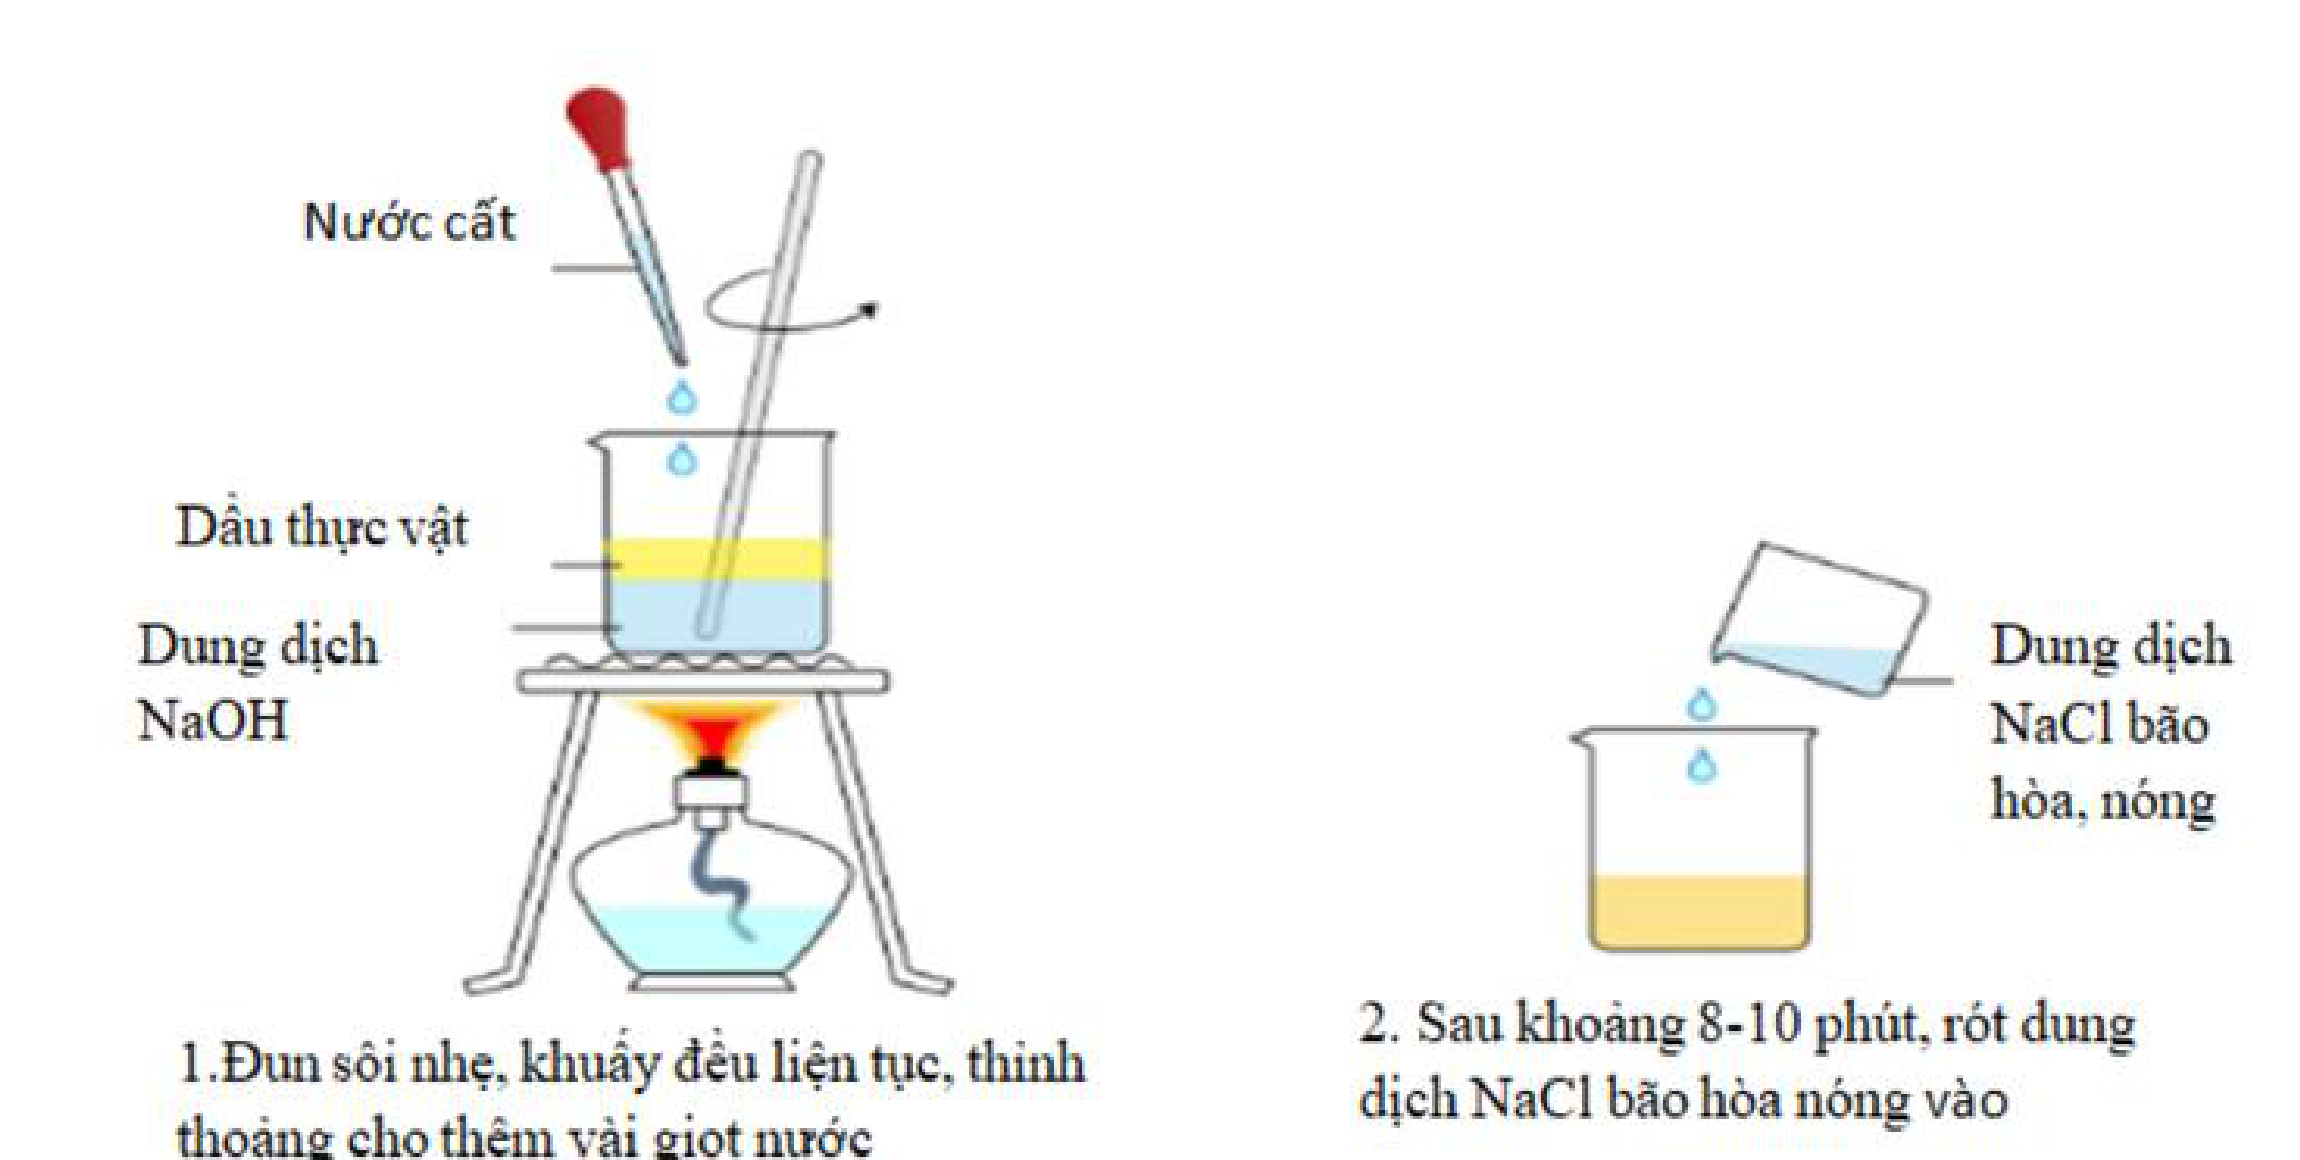
\includegraphics[width=9.5cm]{images_crop_de02/cau2_thi_nghiem_xa_phong_hoa.png}
\end{center}
Sau thí nghiệm, để nguội hỗn hợp trong cốc và quan sát:
\choiceTF[t]
{\True Khi đã nguội, hỗn hợp trong cốc tách thành 2 lớp.}
{\False Dung dịch $\ce{NaCl}$ bão hòa, nóng là xúc tác cho phản ứng xà phòng hóa.}
{\False Khi đã nguội, có một lớp glycerol nổi lên trên bề mặt hỗn hợp.}
{\True Phản ứng xảy ra trong thí nghiệm là phản ứng thủy phân ester trong môi trường kiềm.}
\loigiai{
\begin{itemize}
	\item a) \textbf{Đúng.} Lớp trên là xà phòng đông tụ màu trắng nổi lên; lớp dưới là dung dịch muối, glycerol và kiềm dư.
	\item b) \textbf{Sai.} Dung dịch $\ce{NaCl}$ bão hòa không phải chất xúc tác mà giúp xà phòng kết tinh tách lớp (muối kết).
	\item c) \textbf{Sai.} Lớp nổi lên bề mặt là xà phòng; glycerol tan tốt trong nước ở lớp dung dịch phía dưới.
	\item d) \textbf{Đúng.} Thủy phân triester (chất béo) trong dung dịch kiềm ($\ce{NaOH}$) là phản ứng xà phòng hóa.
\end{itemize}}
\end{ex}

\begin{ex}
Xét các phát biểu về xà phòng và chất giặt rửa:
\choiceTF[t]
{\False Chất kị nước là những chất không tan trong dầu mỡ, hydrocarbon,...}
{\False Muối sodium hoặc potassium của carboxylic acid được dùng làm xà phòng.}
{\True Xà phòng bị giảm hoặc mất tác dụng tẩy rửa khi dùng nước cứng vì gốc acid béo dễ kết tủa với cation $\ce{Ca^{2+}}, \ce{Mg^{2+}}$.}
{\True Xà phòng, chất giặt rửa tan vào nước tạo dung dịch có sức căng bề mặt nhỏ làm cho vật cần giặt rửa dễ thấm ướt.}
\loigiai{
\begin{itemize}
	\item a) \textbf{Sai.} Chất kị nước là chất không tan trong nước nhưng tan tốt trong dầu mỡ, hydrocarbon.
	\item b) \textbf{Sai.} Phải là muối của acid béo (mạch dài từ 12-24C), các acid mạch ngắn không có tính giặt rửa.
	\item c) \textbf{Đúng.} Tạo kết tủa không tan $(\ce{RCOO})_2\ce{Ca}$ và $(\ce{RCOO})_2\ce{Mg}$ làm mất bọt và giảm tính tẩy rửa.
	\item d) \textbf{Đúng.} Phân tử hoạt động bề mặt làm giảm sức căng bề mặt, giúp nước dễ thấm sâu vào sợi vải.
\end{itemize}}
\end{ex}

\begin{ex}
Có bốn ống nghiệm: ống (1) chứa $3\text{ mL}$ nước cất; ống (2) chứa $3\text{ mL}$ nước xà phòng; ống (3) chứa $3\text{ mL}$ nước xà phòng và 3 giọt dung dịch $\ce{CaCl2}$ bão hoà; ống (4) chứa $3\text{ mL}$ nước giặt rửa tổng hợp và 3 giọt dung dịch $\ce{CaCl2}$ bão hoà. Cho vào mỗi ống nghiệm 3 giọt dầu ăn, lắc đều:
\choiceTF[t]
{\False Trong ống nghiệm (1), dầu ăn không tan và chìm xuống dưới.}
{\True Trong ống nghiệm (2), dầu ăn tan tạo hỗn hợp đồng nhất.}
{\True Trong ống nghiệm (3) có kết tủa xuất hiện.}
{\True Trong ống nghiệm (4), dầu ăn tan tạo hỗn hợp đồng nhất.}
\loigiai{
\begin{itemize}
	\item a) \textbf{Sai.} Dầu ăn nhẹ hơn nước ($d \approx 0{,}9\text{ g/mL}$) nên nổi lên trên mặt nước cất.
	\item b) \textbf{Đúng.} Xà phòng nhũ hóa dầu ăn tạo thành hệ nhũ tương bền, đồng nhất.
	\item c) \textbf{Đúng.} Ion $\ce{Ca^{2+}}$ tạo kết tủa trắng với anion acid béo: $2\ce{RCOO^- + Ca^{2+} -> (RCOO)2Ca v}$.
	\item d) \textbf{Đúng.} Chất giặt rửa tổng hợp không bị kết tủa bởi nước cứng nên vẫn nhũ hóa dầu ăn bình thường.
\end{itemize}}
\end{ex}

\vspace{0.3cm}
\noindent
\textbf{PHẦN III (1,5 điểm -- 6 câu): Câu trắc nghiệm yêu cầu trả lời ngắn.}\\
\textit{Thí sinh trả lời từ câu 1 đến câu 6. Mỗi câu hỏi thí sinh điền câu trả lời ngắn gọn theo yêu cầu.}

\setcounter{ex}{0}

\begin{ex}
Cho các chất sau: $\ce{C15H31COONa}$; $\ce{C15H31COOK}$; $\ce{CH3[CH2]11OSO3Na}$; $\ce{CH3[CH2]11C6H4SO3Na}$; $\ce{C17H33COOK}$. Số chất là thành phần chính của chất giặt rửa tổng hợp là bao nhiêu?
\loigiai{
Chất giặt rửa tổng hợp gồm: $\ce{CH3[CH2]11OSO3Na}$ (muối alkyl sulfate) và $\ce{CH3[CH2]11C6H4SO3Na}$ (muối alkylbenzene sulfonate). Các muối còn lại là thành phần của xà phòng. $\Rightarrow$ Có \textbf{2} chất.\\
\textbf{Đáp số: 2.}}
\end{ex}

\begin{ex}
Thuỷ phân hoàn toàn triglyceride X thu được glycerol và 3 acid béo là lauric acid, palmitic acid và oleic acid. X có thể có bao nhiêu công thức cấu tạo?
\loigiai{
Glycerol có 2 vị trí $\alpha$ đối xứng và 1 vị trí $\beta$ ở giữa. Khi gắn 3 gốc acid béo khác nhau vào glycerol, số cấu tạo thỏa mãn là số cách chọn 1 gốc nằm ở vị trí $\beta$: $C_3^1 = \mathbf{3}$ đồng phân.\\
\textbf{Đáp số: 3.}}
\end{ex}

\begin{ex}
Có bao nhiêu hợp chất hữu cơ đơn chức, phân tử chỉ chứa carbon, hydrogen, oxygen và có phân tử khối là 60?
\loigiai{
Phân tử khối $M = 60$ chứa C, H, O:\\
- $\ce{C3H8O}$ có 3 chất: $\ce{CH3CH2CH2OH}$, $\ce{CH3CH(OH)CH3}$, $\ce{CH3CH2OCH3}$.\\
- $\ce{C2H4O2}$ có 2 chất: $\ce{CH3COOH}$, $\ce{HCOOCH3}$.\\
Tổng cộng có $3 + 2 = \mathbf{5}$ hợp chất hữu cơ đơn chức.\\
\textbf{Đáp số: 5.}}
\end{ex}

\begin{ex}
Chỉ số xà phòng hoá là số miligam $\ce{KOH}$ dùng để xà phòng hoá hết triglyceride và trung hoà hết lượng acid tự do trong $1\text{ g}$ chất béo. Một chất béo chứa 3,55\% stearic acid và 89\% tristearin về khối lượng, còn lại là các chất không tham gia phản ứng với $\ce{KOH}$. Tính chỉ số xà phòng hoá của chất béo trên.
\loigiai{
Trong $1\text{ g}$ chất béo:\\
$n_{\text{stearic acid}} = \dfrac{0{,}0355}{284} = 1{,}25 \times 10^{-4}\text{ mol}$; $n_{\text{tristearin}} = \dfrac{0{,}89}{890} = 0{,}001\text{ mol}$.\\
$n_{\ce{KOH}} = 1{,}25 \times 10^{-4} + 3 \times 0{,}001 = 0{,}003125\text{ mol}$.\\
$m_{\ce{KOH}} = 0{,}003125 \times 56 = 0{,}175\text{ g} = \mathbf{175\text{ mg}}$.\\
\textbf{Đáp số: 175.}}
\end{ex}

\begin{ex}
Xà phòng hoá hoàn toàn $0{,}1\text{ mol}$ ester E đơn chức, mạch hở bằng dung dịch $\ce{NaOH}$ vừa đủ thu được muối F và alcohol G. Biết khối lượng muối F thu được lớn hơn khối lượng ester E đã tham gia xà phòng hoá. Tính khối lượng alcohol G thu được (theo gam).
\loigiai{
Phương trình: $\ce{RCOOR' + NaOH -> RCOONa + R'OH}$.\\
$m_{\text{muối}} > m_{\text{ester}} \Rightarrow 23 > M_{\ce{R'}} \Rightarrow \ce{R'}$ là $-\ce{CH3}$ ($M = 15$).\\
Alcohol G là $\ce{CH3OH}$ $\Rightarrow m_{\ce{CH3OH}} = 0{,}1 \times 32 = \mathbf{3{,}2\text{ gam}}$.\\
\textbf{Đáp số: 3,2.}}
\end{ex}

\begin{ex}
Chỉ số xà phòng hóa (SAP): Lượng $\ce{KOH}$ cần thiết (tính bằng miligam) để phản ứng hết với $1\text{ gam}$ dầu, mỡ theo phản ứng xà phòng hóa và trung hòa hết carboxylic acid tự do có trong dầu, mỡ. Trong kĩ thuật, để tính lượng $\ce{NaOH}$ dùng để xà phòng hóa người ta xác định hệ số $a = \dfrac{\text{SAP}}{1402{,}5}$; $m_{\ce{NaOH}} = a \cdot m_{\text{chất béo}}\text{ (gam)}$. Biết loại dầu dừa có giá trị SAP là 255. Tính khối lượng của $\ce{NaOH}$ cần dùng để xà phòng hóa hết $200\text{ gam}$ dầu dừa. \textit{(Kết quả làm tròn đến hai chữ số thập phân)}.
\loigiai{
$a = \dfrac{255}{1402{,}5} \approx 0{,}181818$.\\
$m_{\ce{NaOH}} = \dfrac{255}{1402{,}5} \times 200 \approx \mathbf{36{,}36\text{ gam}}$.\\
\textbf{Đáp số: 36,36.}}
\end{ex}


\bigskip
\begin{center}
	\textbf{\large BẢNG TỔNG HỢP ĐÁP ÁN ĐỀ SỐ 2}
\end{center}

\noindent\textbf{PHẦN I:}
\begin{center}
\begin{tabular}{|c|c|c|c|c|c|c|c|c|c|}
\hline
\textbf{1} & \textbf{2} & \textbf{3} & \textbf{4} & \textbf{5} & \textbf{6} & \textbf{7} & \textbf{8} & \textbf{9} & \textbf{10} \\ \hline
C & A & D & B & D & D & B & A & B & C \\ \hline
\textbf{11} & \textbf{12} & \textbf{13} & \textbf{14} & \textbf{15} & \textbf{16} & \textbf{17} & \textbf{18} & & \\ \hline
B & A & B & A & B & C & A & C & & \\ \hline
\end{tabular}
\end{center}

\noindent\textbf{PHẦN II:}
\begin{center}
\begin{tabular}{|c|c|c|c|c|}
\hline
\textbf{Câu} & \textbf{Ý a} & \textbf{Ý b} & \textbf{Ý c} & \textbf{Ý d} \\ \hline
\textbf{1} & S & S & Đ & S \\ \hline
\textbf{2} & Đ & S & S & Đ \\ \hline
\textbf{3} & S & S & Đ & Đ \\ \hline
\textbf{4} & S & Đ & Đ & Đ \\ \hline
\end{tabular}
\end{center}

\noindent\textbf{PHẦN III:}
\begin{center}
\begin{tabular}{|c|c|c|c|c|c|}
\hline
\textbf{Câu 1} & \textbf{Câu 2} & \textbf{Câu 3} & \textbf{Câu 4} & \textbf{Câu 5} & \textbf{Câu 6} \\ \hline
2 & 3 & 5 & 175 & 3,2 & 36,36 \\ \hline
\end{tabular}
\end{center}

\begin{center}
	\textbf{---------- HẾT ----------}
\end{center}

\end{document}
